\documentclass[12pt]{article}
\usepackage{tikz}
\usetikzlibrary{mindmap}
\begin{document}
\begin{figure}

  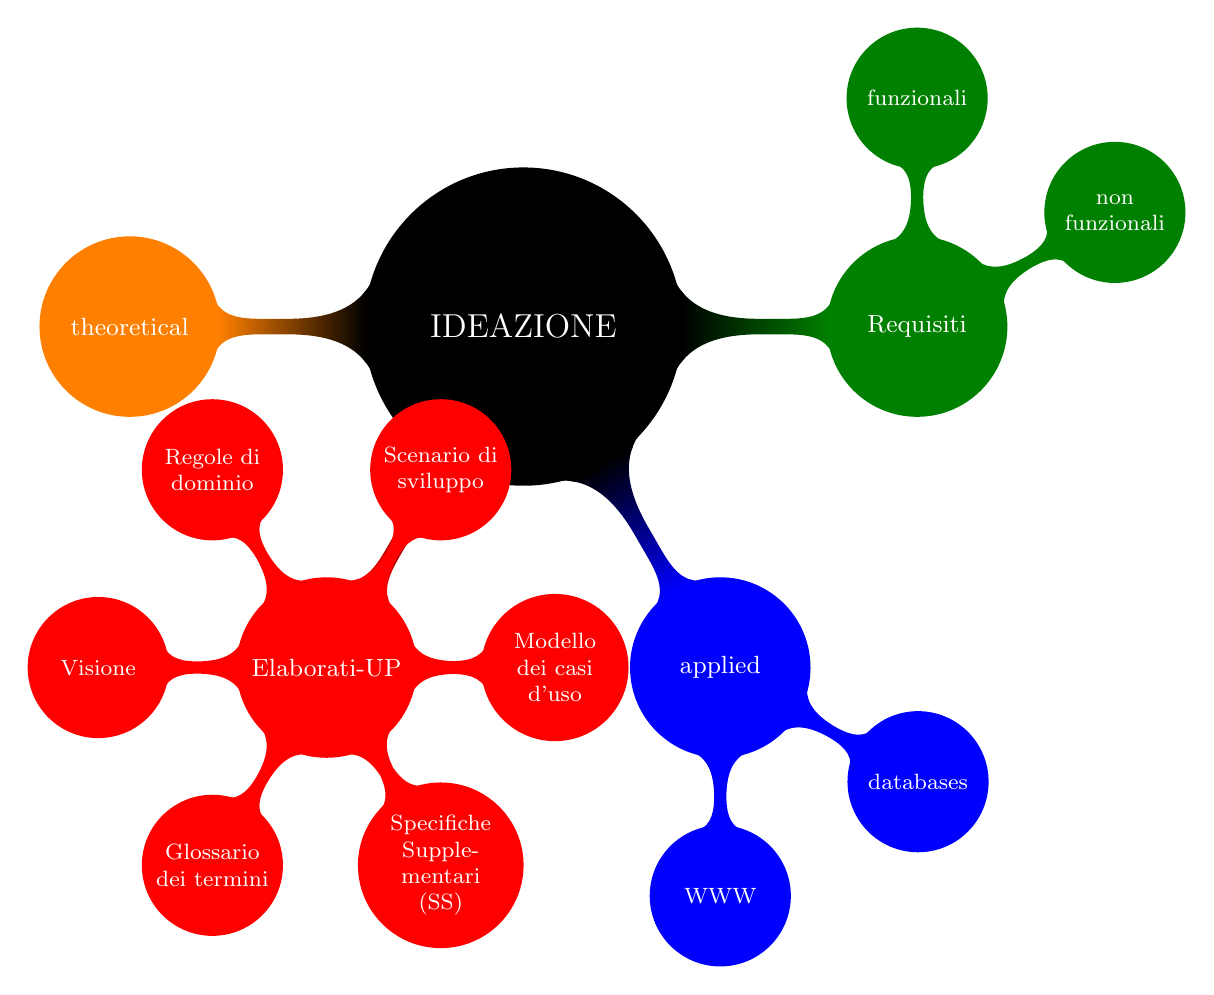
\begin{tikzpicture}
    \path[mindmap,concept color=black,text=white]
    node[concept] {IDEAZIONE}
    [clockwise from=0]
    child[concept color=green!50!black] { node[concept] {Requisiti} [clockwise from=90]
      child { node[concept] {funzionali} }
      child { node[concept] {non funzionali} }
    }
    child[concept color=blue] { node[concept] {applied} [clockwise from=-30]
      child { node[concept] {databases} }
      child { node[concept] {WWW} }
    }
    child[concept color=red] { node[concept] {Elaborati-UP} 
      child { node[concept] {Modello dei casi d'uso} }
      child { node[concept] {Specifiche Supplementari (SS)} }
      child { node[concept] {Glossario dei termini} }
      child { node[concept] {Visione} }
      child { node[concept] {Regole di dominio} }
      child { node[concept] {Scenario di sviluppo} }
    }
    child[concept color=orange] { node[concept] {theoretical} };
    \end{tikzpicture}

\end{figure}
\end{document}